\subsection{Dominant topologies}

The statistics given in Figure~\ref{fig:sbndStats} indicate that the dominant interactions observable in SBND will be CC0$\pi$ and CC1$\pi ^{\pm}$, example Feynman diagrams of the main contributing processes at the free-nucleon level are given in Figure~\ref{fig:feyn}. 

    \begin{figure}[h!]
        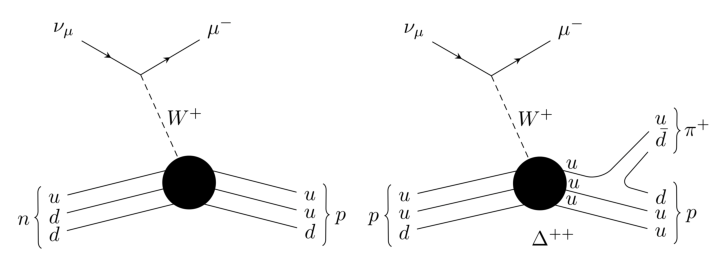
\includegraphics[width=\textwidth]{images/feynmans.pdf}
        \caption{On the left-hand side is a Feynman diagram of the CCQE interaction. During this process, the incoming neutrino interacts with a neutron and produces a muon and a single proton as the observable final state particles. On the right is the postive version of the CC1$\pi ^{\pm}$ interaction, in which a neutrino interacts with a proton emitting a $\pi ^{+}$ alongside the final state muon and proton. Here, the invariant mass of the entire hadronic system must be accounted for when reconstructing the neutrino energy.}
        \label{fig:feyn}
    \end{figure}

One dominant background to the CC0\(\pi\) process is an NC1\(\pi^{\pm}\) interaction, in which the final state pion may decay rapidly into a muon leaving the appearance of a single proton and muon final state as described in equations~(\ref{eq:NC1pi}).

    \begin{equation}
        p + \nu_{\mu} \longrightarrow \nu_{\mu} + p + \pi^{-}
    \end{equation}
    \begin{equation}\label{eq:NC1pi}
        \downarrow
    \end{equation}
    \begin{equation}
        \pi^{-} \longrightarrow \mu^{-} + \bar{\nu}_{\mu}
    \end{equation}

    Backgrounds such as this are an important consideration in all analyses. Though in high resolution detectors such as SBND, the ability to distinguish true signal should be possible to the extent that impurity contributions are minimal. 

\subsection{Energy reconstruction}

    The energy of the incoming neutrino must be reconstructed from the other particles involved in the interaction. When dealing simply with a 2-body hadronic process, such as the one shown in the left hand side of Figure~\ref{fig:feyn}, it is acceptible to use the quasi-elastic estimation~(\ref{eq:Ereco}) \cite{teppei} to calculate the reconstructed energy, $\bar{E}_{\nu}$. Where $E_{\mu}, m_{\mu}$ and $\underline{k}'_{\mu}$ are the energy, mass and 3-momentum of the final state
    muon, $M_{N}$ is the mass of a target nucleon and $\theta$ is the opening angle between the outgoing muon and proton \cite{teppei}.  


    \begin{equation}\label{eq:Ereco}
        \bar{E}_{\nu} = \frac{ E_{\mu} - m^{2}_{\mu} / (2M_{N}) }{ 1 - ( E_{\mu} - |\underline{k}'_{\mu}| cos \theta ) / M_{N} }
    \end{equation}

Alternatively, if the interaction involves more particles in the final state, such as multiple protons or pions escaping the nucleus, one must account for the energy given to all of the hadronic final state particles in the energy reconstruction. 

\subsection{Complications in the free nucleon theory}

Theoretical models of physical interactions on free nucleons are well-grounded, since any incoming particles will interact entirely externally to the particles they collide with. However, when dealing with nuclear targets in high energy physics experiments, such as SBND, complications occur in our understanding of the true nature of the interactions taken place, and data can become inexplicable in comparison with models built on free nucleon cross sections. 

For instance, in the few-GeV energy range, neutrinos will be able to penetrate the argon nucleus and interact with individual nucleons. Therefore, an observation of the CC0\(\pi\) interaction in SBND would not necessarily indicate that a CCQE process took place between the neutrino and nucleon. Pions may be produced initially but be absorbed before ever escaping, thus leaving them invisible to the detector, this is visualised in Figure~\ref{fig:interNuc}.

    \begin{figure}[h!]
        \centering
        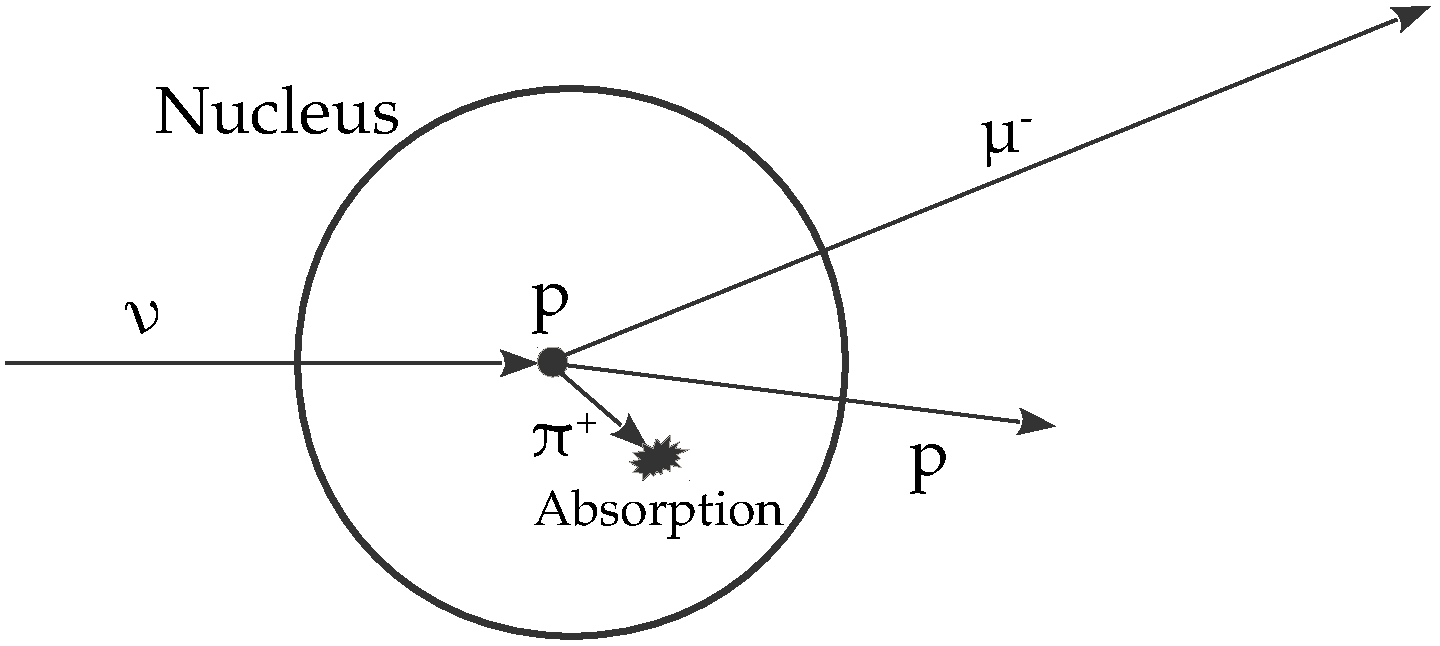
\includegraphics[width=.6\textwidth]{images/inter_nuc.pdf}
        \caption{A schematic of a potential interaction which may occur within the nucleus of an argon atom in SBND, leaving the pion invisible to the detector and the true interaction unidentifiable.}
        \label{fig:interNuc}
    \end{figure}

Another phenomenon that is not accounted for in the free nucleon theory is the potential for multiple nucleons to be involved in the intital scattering process. Such nucleons proceed to leave the nucleus and can appear to be products of an unphysical interaction such as the one in equation~(\ref{eq:fakeMEC}),

    \begin{equation}\label{eq:fakeMEC}
        n + \nu_{\mu} \longrightarrow p + p + \mu^{-}
    \end{equation}

    which is known as the 2-particle 2-hole effect, dominated by the Meson Exchange Current (MEC) \cite{MEC}. When infact, the interaction in equation~(\ref{eq:realMEC}),
    
    \begin{equation}\label{eq:realMEC}
        n + p + \nu_{\mu} \longrightarrow p + p + \mu^{-}
    \end{equation}

    actually occured within the nucleus. \\

    In recent experiments, an excess of scattering events have been observed with respect to the theoretical predictions. It is now believed that MEC could be responsible, and it is therefore a primary concern of theorists, neutrino event generators and nuclear physicists to work together in correctly simulating what may occur in all future neutrino experiments with nuclear targets, in order to overcome these issues \cite{MEC}.

    The region of interest with respect to this excess of scattering events is depicted in Figure~\ref{fig:dipReg} \cite{dipReg}. The point of cross-over between the QE and Inelastic interaction cross sections alone dips significantly, whereas the data indicates that the dip should not be quite as drastic. When adding in the MEC contribution and calculating the total cross section, this dip region increases to fit more closely with the data.  

    \begin{figure}[h!]
        \centering
        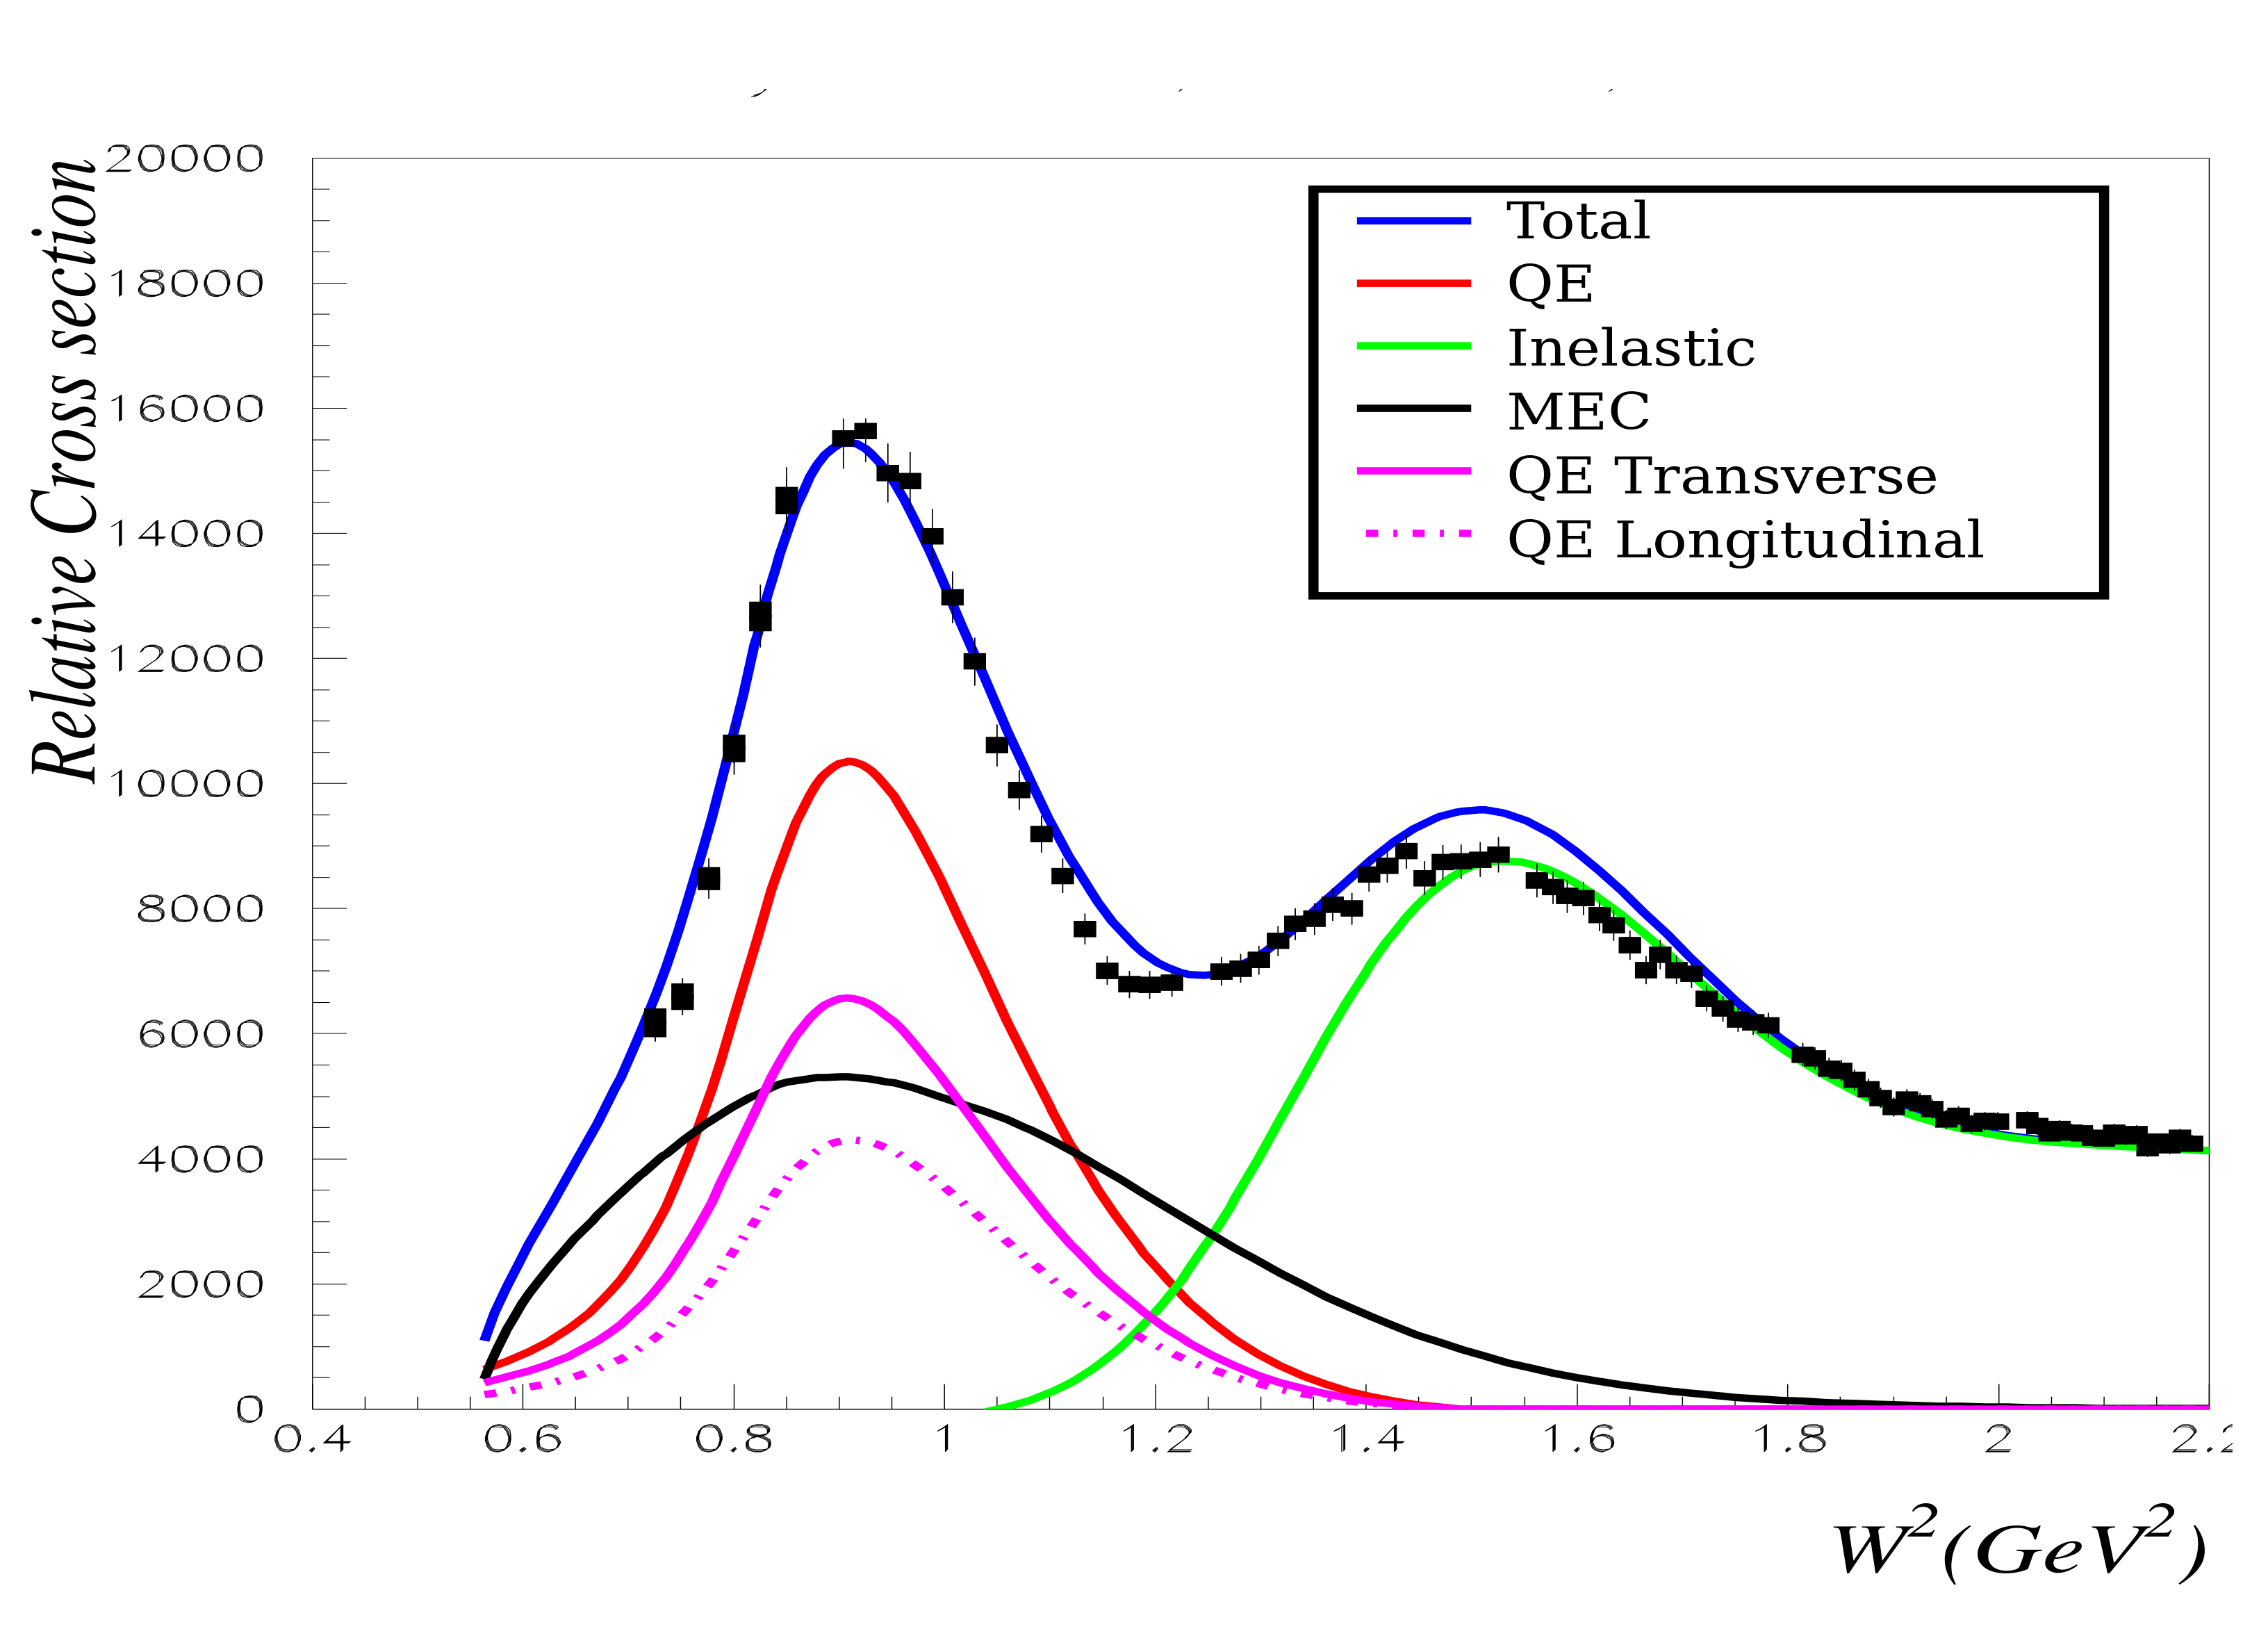
\includegraphics[width=.8\textwidth]{images/dip_region_3.png}
        \caption{The contribution of various interactions to cross section predictions, it is only with the inclusion of MEC that the total cross section comes close to resembling that of data}
        \label{fig:dipReg}
    \end{figure}

    Another indication that MEC is the cause of the observed excess is shown in Figure~\ref{fig:CCQEXsec} \cite{xsecModels}. In this diagram, various theoretical models are shown along with the data obtained. Here, most of the models fit to one another, but their cross sections collectively reside much lower than appears in the data. The closest fitting model to this data is the Martini, LFG+2p2h+RPA model, where 2p2h is the MEC contribution. Though tuning the parameter M\(_{A}\) also improves the RFG fit.  

    \begin{figure}[h!]
        \centering
        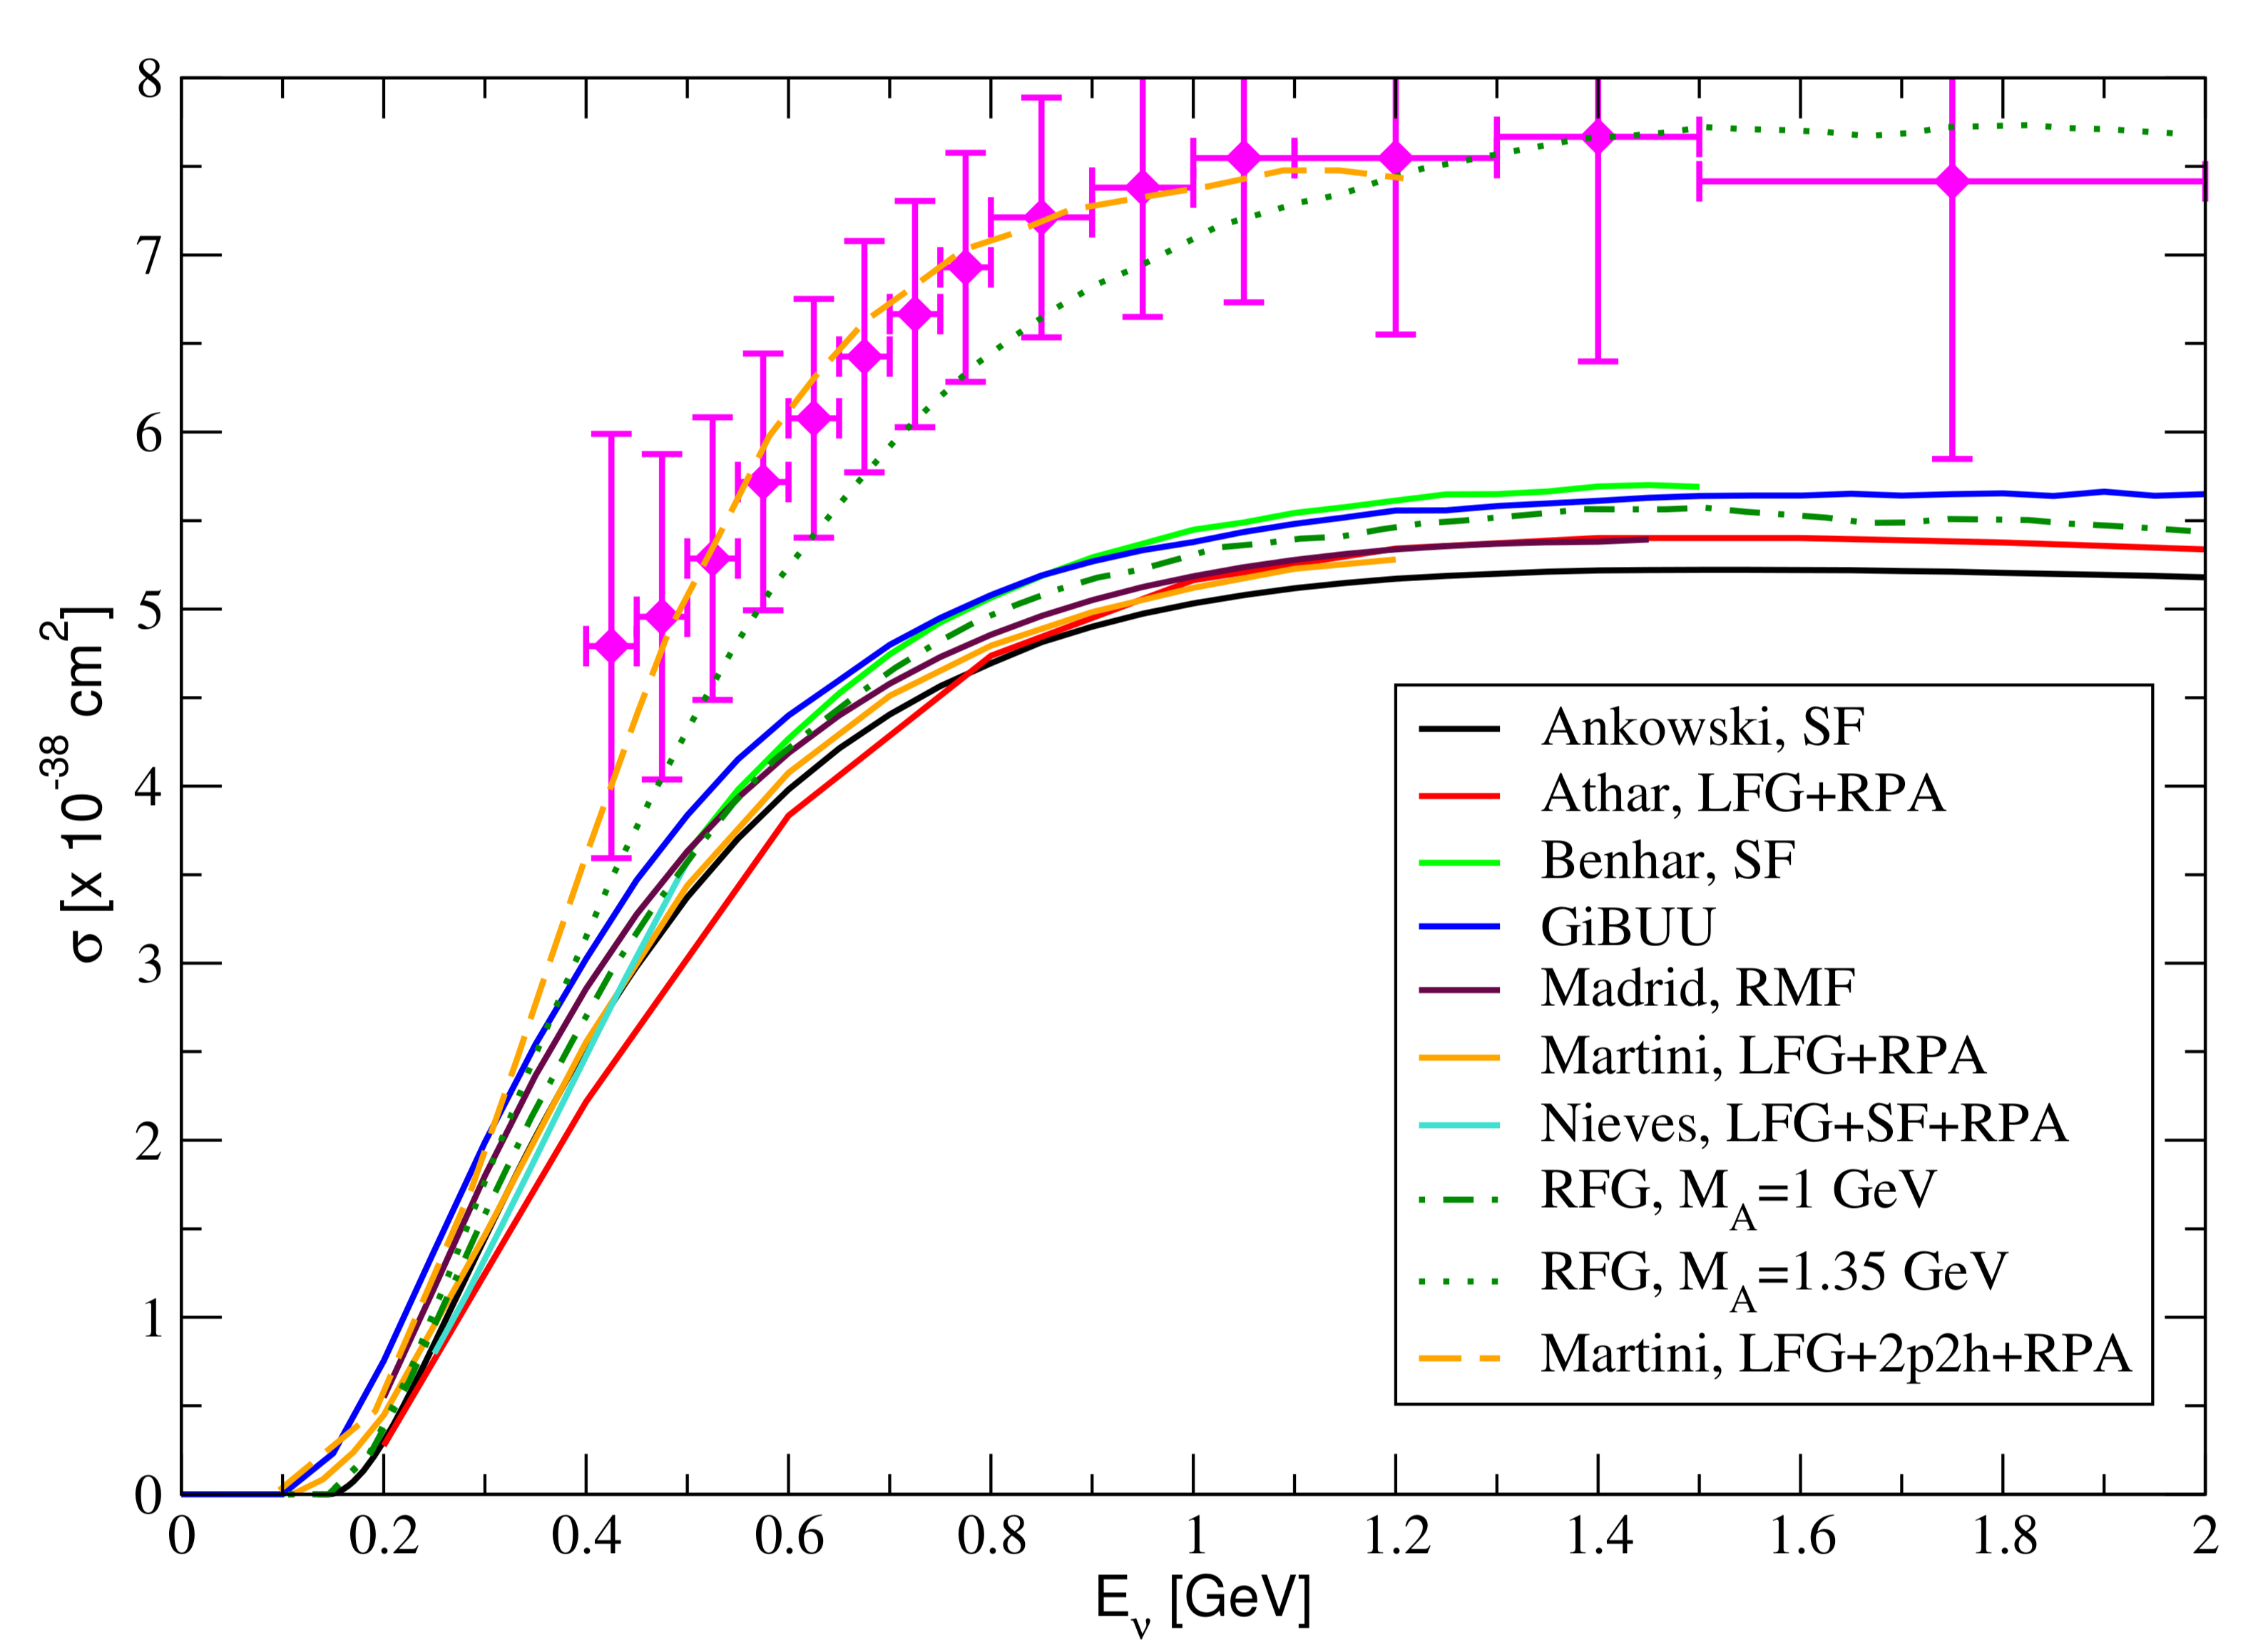
\includegraphics[width=.8\textwidth]{images/CCQE_xsec_2.png}
        \caption{A collection of theoretical predictions made for the CCQE interaction compared with data, once again it is a model with the contribution of MEC which comes closest to correctly predicting the trend of the data, though tuning M\(_{A}\) improves the fit of the RFG model.}
        \label{fig:CCQEXsec}
    \end{figure}

It is therefore clear that constructing model configurations with the correct physical theory is extremely important, but tuning the parameters which make up the models is also a crucial component in building predictions.

\subsection{Preliminary categorisation exercise}

To address these complications in practice, a preliminary exercise was carried out which aimed to characterise the expected initial and final state interactions for the observation of a CC0\(\pi\) event in SBND. Alongside this, the potential backgrounds were also categorised in order to quantify their effect. 

    This exercise also contributed to the initial construction of an anaylsis framework which will eventually be expanded to incorporate fully reconstructed simulations and multiple final state topologies. In the first stage of this exercise however, a MC sample of neutrino events was generated and a manual amount of smearing was applied to them along with energy cuts and an application of pionic impurities in order to loosely represent reconstructed events in SBND whilst training the analysis framework.  

The Monte Carlo sample of SBND events was simulated using the Default+MEC GENIE model and the SBND flux, given in Figure~\ref{fig:SBNDFlux}. The quantites applied to the smearing, impurity additions and energy cuts are as follows, 

    \begin{figure}[h!]
        \centering
        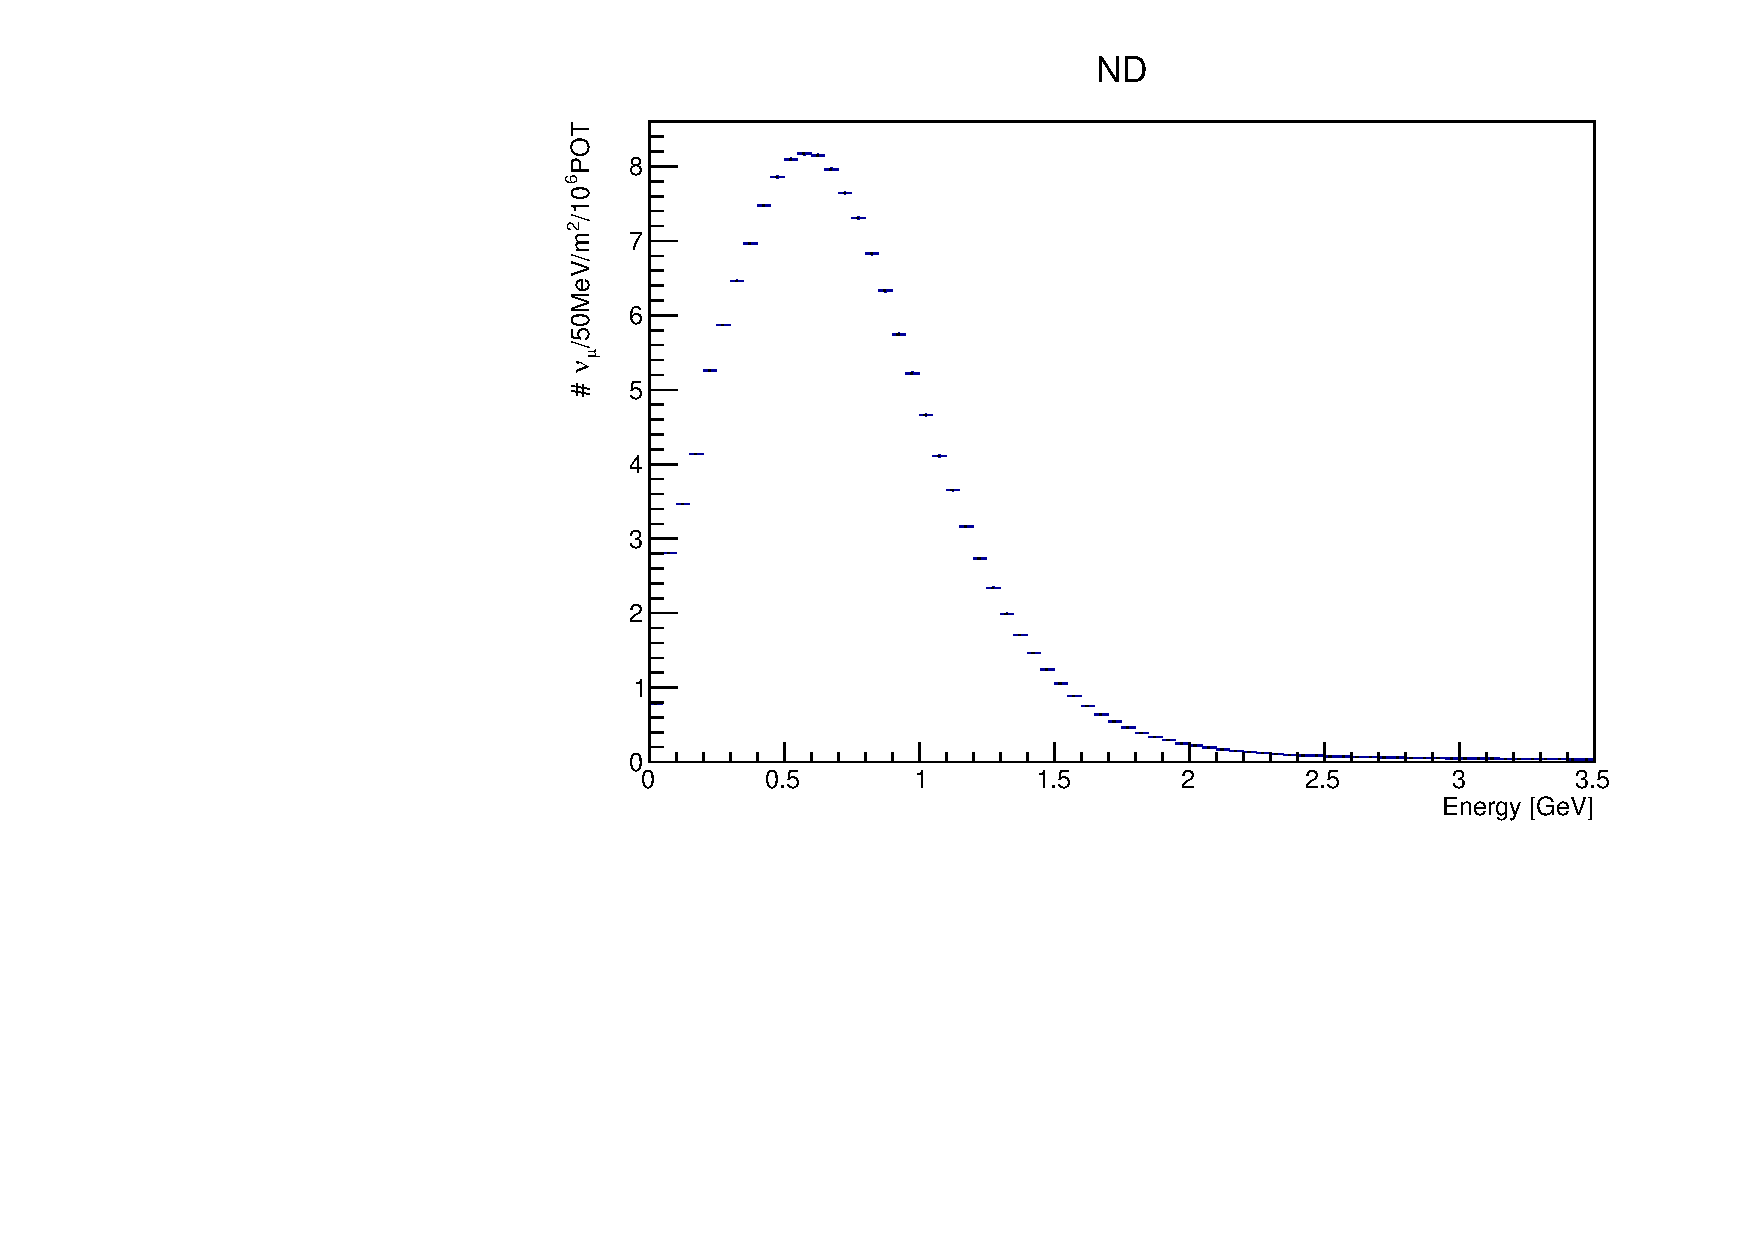
\includegraphics[width=.8\textwidth, trim=0 0 0 1cm, clip]{images/sbnd_flux.pdf}
        \caption{The flux of \(\nu_{\mu}\) at the short baseline near detector used to generate the neutrino events used throughout the following exercise}
        \label{fig:SBNDFlux}
    \end{figure}

\begin{itemize}
    \item Fill after meeting with Ornella
\end{itemize}

These quantities were calculated using the following SBND geometry and energy resolution information,

\begin{itemize}
    \item Fill after meeting with Ornella
\end{itemize}

In a CC0\(\pi\) interaction, the potential backgrounds within the detector will contaminate the signal for various reasons including:

\begin{itemize}
    \item Low energy energy depositions of pions
    \item Mis-identification of pions
    \item ...
\end{itemize}

In this exercise, both the signal and background were split into potential contributing topologies in order to highlight the interaction characteristics within the detector and identify the channels which will be of interest in SBND. 
   
One potential extention to this exercise would be to compare the smeared/reconstructed predictions with existing data to draw comparisons in a more realistic situation. The chosen experiment for this is MiniBooNE, which had the same baseline and energy range as SBND will have. For this reason, the kinematics studied were the same as that of MiniBooNE: muon kinetic energy as a function of the opening angle of the final state particles. An example comparison between
MiniBooNE data and predictions made by GENIE is shown in Figure~\ref{fig:MBComp}. The binning was also replicated in this exercise for the same reasons.


    % Plan
    \begin{itemize}
        \item RESULTS
        \item This will be better implemented in LArSoft using full detector simulation
        \item Efficiency and purity definitions for the detector
    \end{itemize}


\clearpage
